\author{Florian Müller}
\section {Preprocess images for the AI}

\texttt{text = letter\_slicer(image, roi, task\_types)}

The main function to preprocess the images which include text is \texttt{letter\_slicer()}.
This function receive three attributes and returns a string with the found letters.
The first attribute is the original image followed by the region of interesst as coordinates.
The last attribute is the task\_type which determines which model will be used for the detection.

In the beginning the dynamic letter high and erosion value is calculated.
Then the region of interesst is cut out of the original image.

\begin{figure}[H]
    \centering
    \subfloat{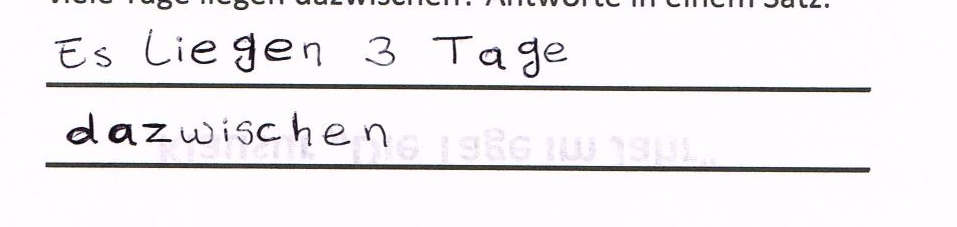
\includegraphics[width=0.6\linewidth]{src/chapters/developer/media/ld_live/ld_roim.png}}
    \caption{Region of interesst}
\end{figure}

The region of interesst is converted to grayscale.

\begin{figure}[H]
    \centering
    \subfloat[][]{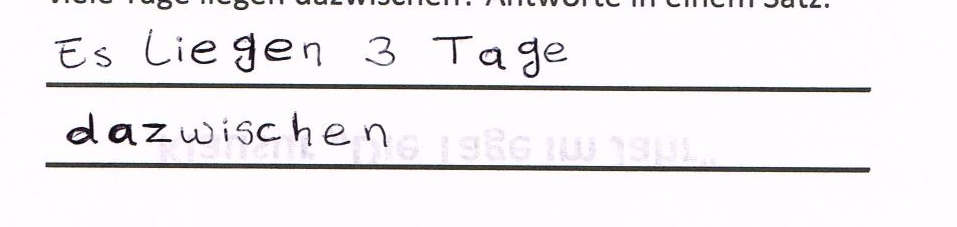
\includegraphics[width=0.4\linewidth]{src/chapters/developer/media/ld_live/ld_roim.png}}
    \qquad
    \subfloat[][]{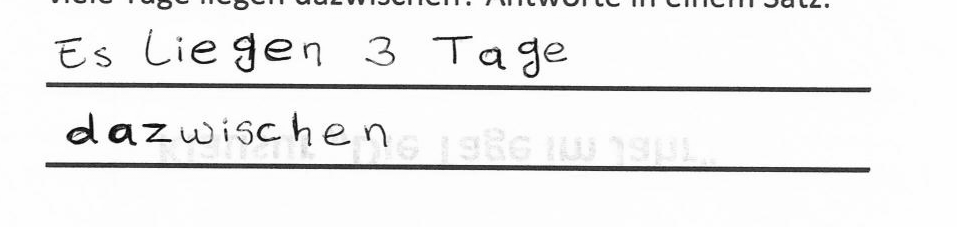
\includegraphics[width=0.4\linewidth]{src/chapters/developer/media/ld_live/ld_gray.png}}
    \caption{From original(a) to grayscale(b)}
\end{figure}

Then the grayscale image will be thresholded to reduce noise.

\begin{figure}[H]
    \centering
    \subfloat[][]{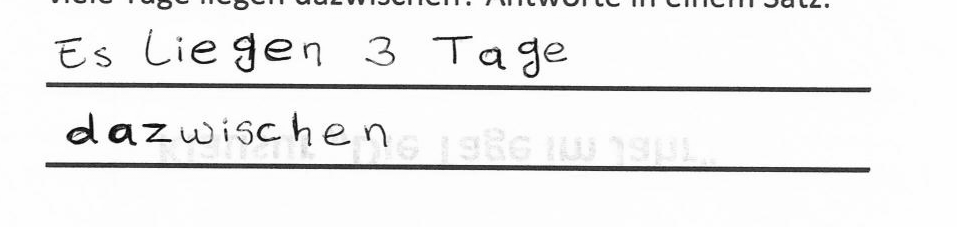
\includegraphics[width=0.4\linewidth]{src/chapters/developer/media/ld_live/ld_gray.png}}
    \qquad
    \subfloat[][]{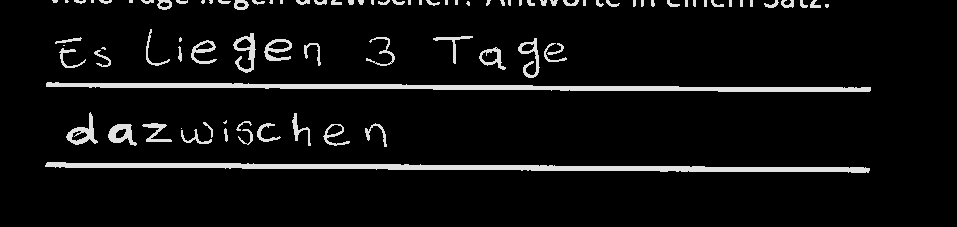
\includegraphics[width=0.4\linewidth]{src/chapters/developer/media/ld_live/ld_thresh.png}}
    \caption{From grayscale(a) to thresholded(b)}
\end{figure}

After that an erosion is applied to the thresholded image to get rid of the rest of the noise.

\begin{figure}[H]
    \centering
    \subfloat[][]{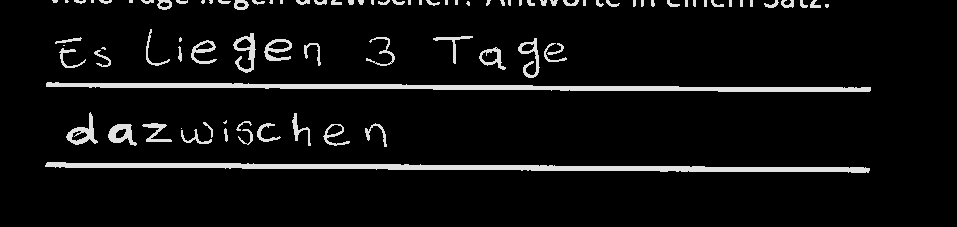
\includegraphics[width=0.4\linewidth]{src/chapters/developer/media/ld_live/ld_thresh.png}}
    \qquad
    \subfloat[][]{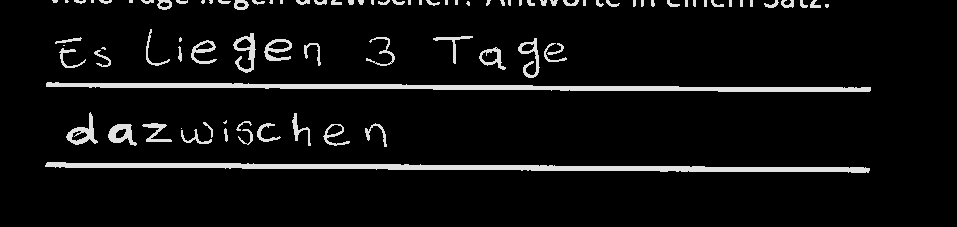
\includegraphics[width=0.4\linewidth]{src/chapters/developer/media/ld_live/ld_erode01.png}}
    \caption{From threshold(a) to eroded(b)}
\end{figure}

To find the seperated lines the image will be dilated horizontaly to create a big block flor each line.

\begin{figure}[H]
    \centering
    \subfloat[][]{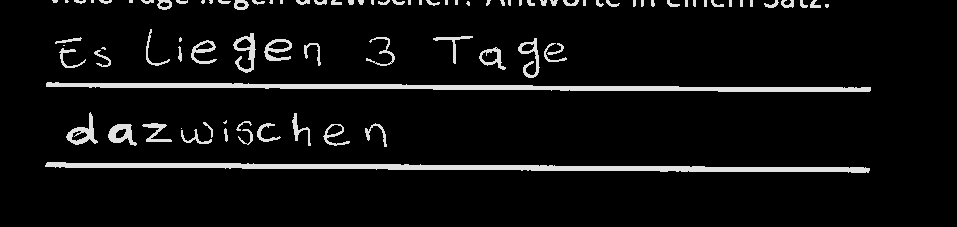
\includegraphics[width=0.4\linewidth]{src/chapters/developer/media/ld_live/ld_erode01.png}}
    \qquad
    \subfloat[][]{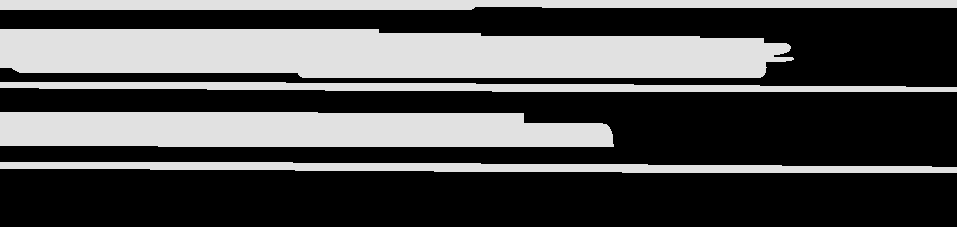
\includegraphics[width=0.4\linewidth]{src/chapters/developer/media/ld_live/ld_dilate01.png}}
    \caption{From eroded(a) to dilated lines(b)}
\end{figure}

Now each line can be analysed seperatly.

\texttt{line\_list = letters\_from\_line(image, roi, task\_types, erosion\_val)}

The letters from line funciton receives the region of interesst as image. The \texttt{rio} are the coordinates for each line and the \texttt{erosion\_val} is already calculated in the first function.
Next is to cut the line from the thresholded image.

\begin{figure}[H]
    \centering
    \subfloat[][]{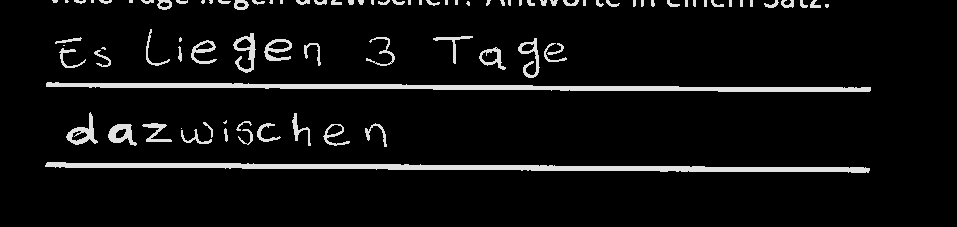
\includegraphics[width=0.4\linewidth]{src/chapters/developer/media/ld_live/ld_thresh.png}}
    \qquad
    \subfloat[][]{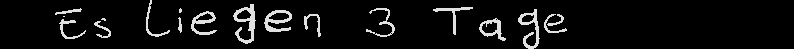
\includegraphics[width=0.4\linewidth]{src/chapters/developer/media/ld_live/line10000.png}}
    \caption{From the thresholded image(a) cut the line(b)}
\end{figure}

Now the line gets an erode applied.

\begin{figure}[H]
    \centering
    \subfloat[][]{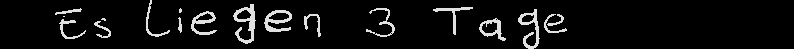
\includegraphics[width=0.4\linewidth]{src/chapters/developer/media/ld_live/line10000.png}}
    \qquad
    \subfloat[][]{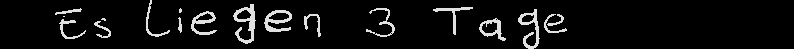
\includegraphics[width=0.4\linewidth]{src/chapters/developer/media/ld_live/line_erode10001.png}}
    \caption{From the line(a) to the eroded line(b)}
\end{figure}

From the eroded line the upper two thirds will be dilated downwards by using a vertical kernel with an anchor on the top position.

\begin{figure}[H]
    \centering
    \subfloat[][]{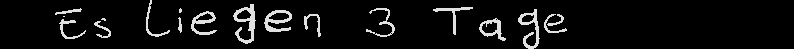
\includegraphics[width=0.4\linewidth]{src/chapters/developer/media/ld_live/line_erode10001.png}}
    \qquad
    \subfloat[][]{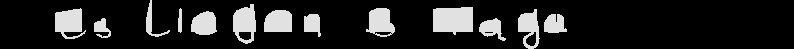
\includegraphics[width=0.4\linewidth]{src/chapters/developer/media/ld_live/dilateline10003.png}}
    \caption{From the eroded line(a) dilate the upper two thirds(b)}
\end{figure}

The dilated line gets a blur applied and the contours are calculated.

\begin{figure}[H]
    \centering
    \subfloat[][]{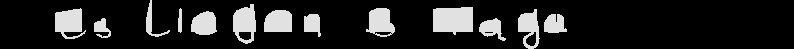
\includegraphics[width=0.4\linewidth]{src/chapters/developer/media/ld_live/dilateline10003.png}}
    \qquad
    \subfloat[][]{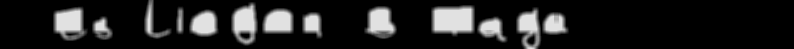
\includegraphics[width=0.4\linewidth]{src/chapters/developer/media/ld_live/blur_dilate_line10004.png}}
    \caption{From the dilated line(a) to the blured dilated line(b)}
\end{figure}

Now for each contour a mask will be created.
Each mask is bitwise added via "and" with the line.
Now the individual character can be cut out, blured and forwarded to the AI interface.

\begin{figure}[H]
    \centering
    \subfloat[][]{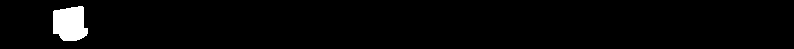
\includegraphics[width=0.4\linewidth]{src/chapters/developer/media/ld_live/mask10005.png}}
    \qquad
    \subfloat[][]{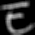
\includegraphics[width=0.2\linewidth]{src/chapters/developer/media/ld_live/blur_letter10006.png}}
    \caption{From the dilated line(a) to the blured dilated line(b)}
\end{figure}

This process is looped over each letter and ech line.
After every letter was detected and analysed the resulting string will be returned.
